\section{Response Time}
Response time is another major feature exploited in Internet traffic analysis attack. Again we would expect the same attacks can be applied to 6LoWPAN traffic and works even better than their counterparts against Internet traffic, as the accuracy of timing measurements can be greatly improved for 6LoWPAN traffic. 

Firstly, the devices are physically close to each other and uses RF to communicate. The adversary can remove the RTT noises by measure the packets on the server side. 

Secondly, performance of the constrained devices are low; hence gives a better resolution on timing code execution.

\subsection{Different Sensors}
%Plaintext recovery.
%\begin{itemize}
%	\item Reading different sensors takes different time.
%	\item Requirement: needs to identify CoAPS packets.
%	\item Works on both 802.15.4 Seuciryt and DTLS, if the requirement is met. 
%\end{itemize}

CoAP\cite{rfc7252} is a protocol designed for constraied devices that provides an universal interface for accessing resources. CoAPs is the secure version which stands for CoAP with DTLS.

Due to the different physical characters of sensors, there could be a variance of time when reading the measurements. The idea is to investigate whether such variance can be observed through the packet response latency.

We implemented the experiment on CC2538, using all three sensors from ``cc2538-demo", namely Vdd, temperature and Ambient Light Sensor (ALS). We used CoAP from the ``er-rest-example" in the Contiki OS source code, as there is no CoAPs implementation available. 

Although DTLS processing would definitely have an impact on the response latency, we argue that such impact would be independent to the sensors being accessed; hence similar result would hold even in case of CoAPs.

We have carefully crafted other factors, including URIs, data representation and code flow, to be uniform for all three sensors in order to guarantee a controlled environment.

\begin{table}
	\center
	\begin{tabular}{|c|c|c|}
	\hline
	& Average (ms) & Range(ms) \\ 
	\hline
	Vdd & 9.622 & [9.388, 10.318] \\ 
	\hline
	Temperature & 9.835 & [9.525, 10.318] \\ 
	\hline
	ALS & 11.651 & [11.338, 12.031] \\
	\hline
\end{tabular} 
	\caption{CoAP Response Latency for Sensor Readings on CC2538\label{CoapTiming}}
\end{table}

\Cref{CoapTiming} summarises the result. It is shown that ALS takes about $2$ms longer and hence can be easily distinguished. Vdd and temperature might be difficult to distinguish by response latency as they have similar results.



\subsection{Different Hardware}
%Gain hardware information.
%\begin{itemize}
%	\item Different hardware has different response latency against the same message.
%	\item For 802.15.4: Requires additional information. Can be satisfied by the previous ICMP attack.
%	\item For DTLS: No requirement. The adversary can actively send a message, e.g. PING.
%\end{itemize}

A more general leakage is the response latency to a specific message, as different processors would have different computational power and thus different time to process a same message. The ICMP messages turns out to be suitable for this attack since they are standardised and thus universally supported. Among the ICMP messages, PING is especially ideal for two reasons: 
\begin{enumerate}
	\item It is mandatory in the ICMP standard.
	\item It only swaps the source and destination address of the packet; thus minimises different code path in protocol processing.
\end{enumerate}

\begin{table}
	\center
	\begin{tabular}{|c|c|c|}
	\hline
			& CC2538	& TelosB \\ 
	\hline
	Average(ms)	& 9.56		& 17.03 \\ 
	\hline
	Range(ms)	& [9.16, 10.06]	& [16.49, 17.68]	\\
	\hline
\end{tabular}

	\caption{PING Response Latency\label{PingResponse}}
\end{table}

\Cref{PingResponse} shows the PING response latency on CC2538 and TelosB. The result confirms that these devices can be distinguished by PING response latency.

\subsection{Running Code Fingerprint}
%Fingerprints the code running on a device, which leads to plaintext recovery.
%\begin{itemize}
%	\item Theory explained in \Cref{FingerprintTheory}.
%	\item Requirement: needs to actively send messages. Any Request/Response protocol works, such as PING, DTLS Heartbeat, CoAP PING, etc. 
%	\item Not for 802.15.4: adversary can't join the network.
%	\item For DTLS: PING is available and confirmed. DTLS Heartbeat should work if supported.
%\end{itemize}
The response time of packets could also be exploited to fingerprint the code running on a specific device. 

\subsubsection{Hypothesis}
%How it works
\Cref{FingerprintTheory} hypothesises two sensors receiving a service request. The first node was idle and hence responded immediately, whilst the second postponed the request for reading a sensor. As a result, the response time on the second sensor would appear to be longer than the first sensor. This scenario applies to the majority of constrained devices as they are mostly single-cored. 

\begin{figure}
	\center
	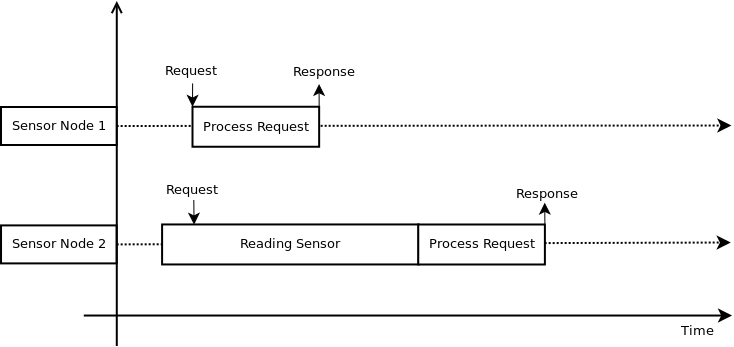
\includegraphics[width=\textwidth]{fig/PingProbe_Theory.png}
	\caption{Variations in Response Time\label{FingerprintTheory}}
\end{figure}

Most sensors are programmed to run in a loop. The idea of code fingerprinting exploits the fact that each program delays the request differently; thus statistically each program results into a distinctive distribution of delayed response time. 

\begin{definition}
	We refer the distribution of delayed response time as a \textbf{``fingerprint''} to the program running on the sensor node.
\end{definition}

We assume the adversary has the pre-knowledge of potential programs, together with a database of all their fingerprints. To identify an unknown program, the adversary collects its fingerprint and then searches the database for a match.

%What can be the Request
To effectively launch the attack, the requests needs to be actively sent by the adversary. Since code information is actually contained in extended  length of response time; therefore requests with short constant processing time are preferable as they induce less noise. In practice, the request can be instantiated by several messages defined in the sensor network protocols. PING is ideal as it induces only negligible computation and is compulsory according to the ICMP standard\cite{rfc4433}. Other options include Heartbeat message in DTLS\cite{rfc6520}, Reset in CoAP\cite{rfc7252}, etc.

\subsubsection{Extracting Fingerprint}
%Experiment Result
We measured PING response time on CC2538 running Contiki OS. Since Contiki MAC\cite{ContikiMAC} sends duplicated PING requests, we define the PING Response Interval, PRI, to be the time between a PING response and its last paired request. 

\Cref{ExamplePri} shows an example where Packet 205 and Packet 203 constitute a pair of PING packets, and their PRI is computed as their difference in time.

\begin{figure}[!h]
	\centering
	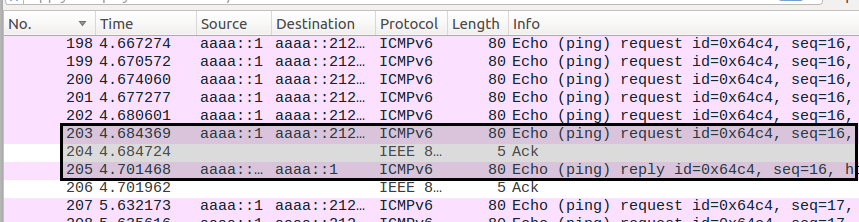
\includegraphics[width=\textwidth]{fig/PRI_hl.png}
	\caption{Example PRI\label{ExamplePri}}
\end{figure}

%Since the attack extracts the information contained in the extended response time of a specific request, the first problem is to see whether such extended response time can be filtered from normal ones. 

\Cref{HelloworldPri} shows the histogram of PRIs collected on ``helloworld'' example from Contiki OS. Values $\geq$12ms are collected at 12ms. The result shows that the majority of PRIs are clustered around 9.5ms, whilst a clear gap exists between the majority and the outliers. The majority, roughly ranged [9.0, 10.3]ms, corresponds to the case of Sensor Node 1 in \Cref{FingerprintTheory}. 

\begin{figure}[!h]
	\centering
	\begin{subfigure}{0.45\textwidth}
		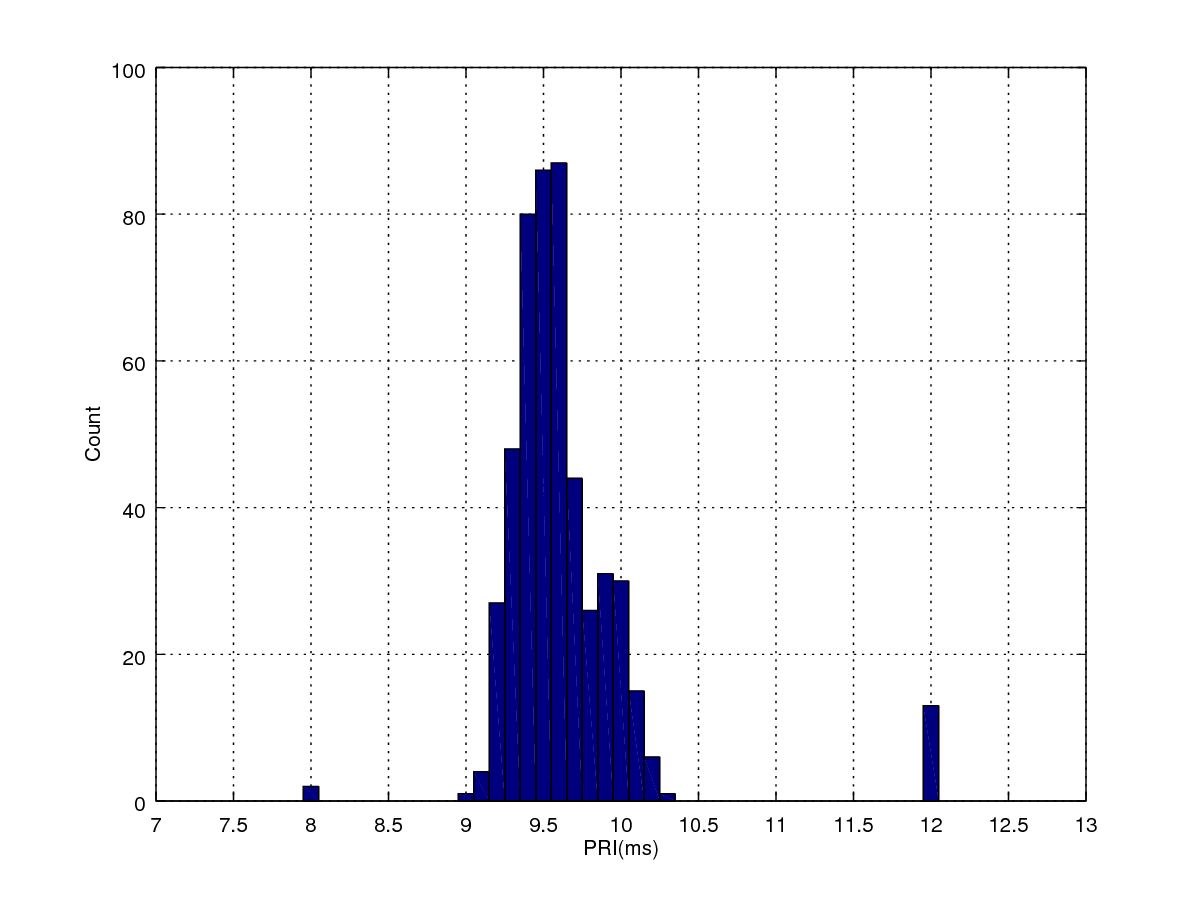
\includegraphics[width=\textwidth]{fig/helloworld_cc2538.png}
		\caption{PRIs of helloworld\label{HelloworldPri}}
	\end{subfigure}
	\begin{subfigure}{0.45\textwidth}
		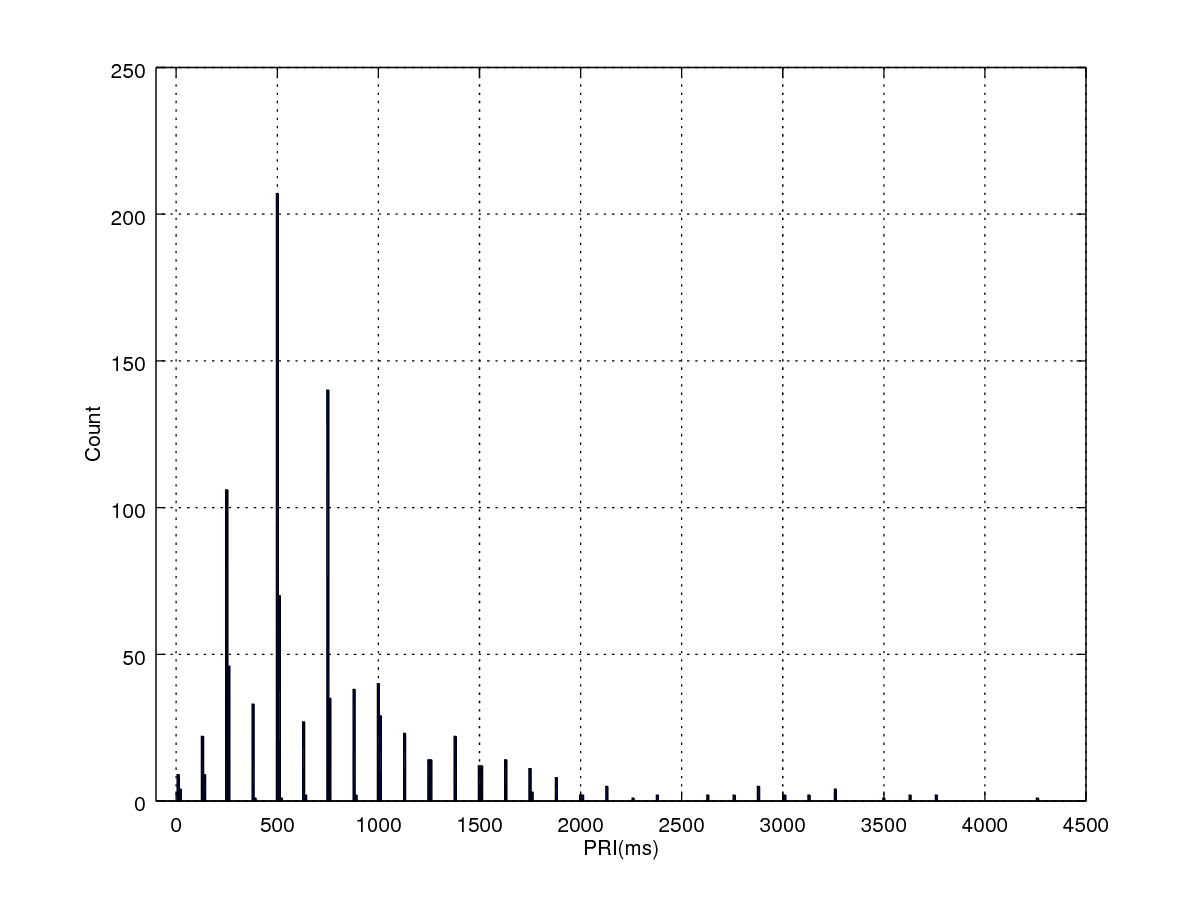
\includegraphics[width=\textwidth]{fig/helloworld_cc2538_outlier.png}
		\caption{PRIs outliers of helloworld\label{HelloworldPriOutliers}}
	\end{subfigure}
	\caption{PRIs for helloworld}
\end{figure}

We further plotted the upper outliers, which mostly ranged from [12, 2000]ms, in \Cref{HelloworldPriOutliers}. We suppose these outliers corresponds to the case of Sensor Node 2 in \Cref{FingerprintTheory} which PING request arrived when the processor was performing another task.

PRIs we collected on other applications showed the same characteristic. The majorities are clustered near a medium value. A clear proportion of outliers exists, leaving a clear gap between the majority. This implies that an adversary can easily draw a threshold by observing the whole distribution and then filter the extended ones out. In our experiments the threshold is set to 12ms but any other values within the gap would also work. 

According to the hypothesis, the  distribution shown in \Cref{HelloworldPriOutliers} is due to different tasks delays the PING request differently. According to the hypothesis


\subsubsection{Fingerprint Matching}
%Comparing the distribution.
Following the hypothesis, we expect a distinctive outlier PRI distribution for each different program running on the target device which can be used as a fingerprint to the program being ran. To identify an unknown program r
